\chapter{Constructing and Testing Circuits}
\label{chapConstructingTesting}

%% FIXME - show examples of connected and unconnected wires, and components placed wrongly if I haven't done so already.

In the previous chapter, we learned the theory behind how to analyze circuits.
In this chapter, we are going to put real circuits together and use simple equipment to analyze the same kinds of problems, and compare our calculated answers to the measurements we make on live circuits.

\section{The Solderless Breadboard}

The most important piece of equipment to use for making circuits is the \glossterm{solderless breadboard}.
Before solderless breadboards, if you wanted to put together a circuit, you had to attach them to a physical piece of wood to hold them down, and then \glossterm{solder} the pieces together.
Soldering is a process where two wires are physically joined using heat and a type of metal called solder, which melts at much lower temperatures than other types of metal.
So, what you would have to do is attach the electrical components to the board, wrap the components' legs around each other, and then heat them up with a soldering iron and add solder to join them permanantly.

This was an involved process, and, though it was possible to get your components back, you were generally stuck with your results.
The solderless breadboard is an amazing invention that allows us to quickly and easily create and modify circuits without any trouble at all.
Figure~\ref{figSolderlessBreadboard} shows what a solderless breadboard looks like.

\simplegraphicsfigure{A Solderless Breadboard}{SolderlessBreadboard}{0.5}

The solderless breadboard has a number of spring clips (usually about 400 or 800 of them) called \glossterm{connection points} which will allow you to insert wires or component leads and will hold them in place.
Not only that, the breadboard itself will connect the components for you!

The way that this works is that the breadboard is broken up into little half-rows called \glossterm{terminal strips}.
Each terminal strip has multiple connection points---usually five.
Each connection point on a given terminal strip is connected by wire \emph{inside} the breadboard.
Therefore, to connect two wires or leads together, all you need to do is connect them to the same terminal strip.
Any two wires or leads connected to the same terminal strip are themselves connected.

In most breadboards, the two sides of the breadboard are separated by a gulf known as the \glossterm{bridge}.
The bridge is a visual indication that the two sets of terminal strips are not connected, but it also serves a practical purpose.
If you have an integrated circuit (a small chip), the bridge is the right width so that you can place your integrated circuit right over the bridge, and each leg of the chip will receive its own terminal strip for you to easily connect them to what you need.
We will cover this in more depth in later chapters.

\simplegraphicsfigure{Parts of a Solderless Breadboard}{SolderlessBreadboardParts}{0.5}

In addition to the terminal strips, most breadboards have two strips running down each side, one with a red line and one with a blue line.
These are known as \glossterm{power rails} (some people call them \glossterm{power buses}).  

Power rails are very similar to terminal strips, with a few exceptions.
The main difference is that, in terminal strips, only the five connection points grouped together are connected.
On power rails, many more of the connection points are connected together, even when there are short gaps.
Some boards will split the power rails at the halfway point, but others go all the way down the board.  
This is usually visually indicated by a break in the red and blue lines that indicate the power rails.

Note that the positive and negative are \emph{not} connected to each other (that would create a short circuit), and they are \emph{not} connected to the power rails on the other side of the breadboard (unless you connect them manually).
As we mentioned, on some breadboards, even a single side isn't connected all the way down, but may be broken into sections at the halfway point.

In many projects, many components need direct access to the positive or negative power supply.
Power rails make this easy by providing a connection point with positive and negative power a very short distance away from wherever you need it on the breadboard.
If you plug your power source's positive and negative terminals into the positive and negative rails on the breadboard, then any time you need a connection to the positive or negative terminal, you can just bring a wire to the closest connection point on the appropriate power rail.

\section{Putting a Circuit Onto a Breadboard}

To see how a simple circuit works on a breadboard, let's go back to the circuit we first looked at in Chapter~\ref{chapFirstCircuit}.
Figure~\ref{figCircuitBasicLEDRepeat} has the drawing again for ease of reference.

\begin{figure}
\caption{Basic LED Circuit}
\label{figCircuitBasicLEDRepeat}
\centering

\includegraphics[scale=0.125]{CircuitBasicLED.png}
\end{figure}

So, how do we translate what we see in the drawing to what we need to put in the breadboard?
Well, let's take a look at what is in the circuit---a 9-volt battery, a LED (we will go with a red LED), and a $1,000\myohm$ resistor.
Let us not concern ourselves with the battery at the moment.
So, without the battery, we have a resistor connected to an LED.

Let us start out by simply placing our components onto the breadboard.
What you will want is to place them on the breadboard so that each of their legs are on \emph{different} terminal strips.
It doesn't matter \emph{which} terminal strips you use---just make sure the legs all get plugged into different ones.
Figure~\ref{figBreadboardBegin} shows how your breadboard should look so far.
Note that the longer leg of the LED is closer to the resistor.

Figure~\ref{figBreadboardBadEdited} shows the \emph{wrong} way to do it.
In that figure, the both of the legs of the components are on the same row, which is the same thing as placing a wire between the legs, creating a short circuit.
Don't do that!  Make sure each leg goes into its own row.

\simplegraphicsfigure{Putting the Components onto the Breadboard}{BreadboardBegin}{1}

\simplegraphicsfigure{The Wrong Way to Put Components onto the Breadboard}{BreadboardBadEdited}{1}

Now, to connect the resistor to the LED, we need to add a wire.
So, all we need to do is connect a wire to any empty connection point that is on the same terminal strip of the right leg of the resistor, and connect the other side of that wire to the left leg of the LED as shown in Figure~\ref{figBreadboardBeginTwo}.

\simplegraphicsfigure{Adding a Wire to Connect the Components}{BreadboardBeginTwo}{1}

A common mistake that people will make is to connect the wire to the row right before or after the component.
Take some time and be extra certain that the wire is connected to the same row as the leg of your components.

Now, we need to connect our project to the power rails.
So, take a red wire from the left leg of the resistor to the positive power rail (remember, as long as it is in the same terminal strip as the resistor, they will be connected).
Likewise, take a black wire from the right leg of the LED to the negative power rail.
I always use red wires for connecting to the positive power rail, and black wires for connecting to the negative/ground rail, as it makes it more clear when I am looking at my project what wire carries what.
Your project should look like Figure~\ref{figBreadboardBeginThree}.

\simplegraphicsfigure{Adding Wires to the Power Rails}{BreadboardBeginThree}{1}

Now your project is almost done.
All you need to do now is to connect your power rails to a power supply.
Connect a T-connector to a 9-volt battery, and then connect the red (positive) wire to the positive power rail on the breadboard.  You can plug it in anywhere on the rail, but I usually connect the power to the edge of the rail to leave more room for components.
Then, connect the black (negative) wire to the negative power rail on the breadboard.
As soon as you do this, the LED should light up!
Figure~\ref{figBreadboardBeginFour} shows the final circuit.

\simplegraphicsfigure{Final LED Circuit with Power Connected}{BreadboardBeginFour}{1}

Note that many T-connectors for 9-volt batteries have very flimsy wires that are difficult to insert into a breadboard.
Usually, as long as you can get both terminals in far enough to touch the metal within the connection point, it will work.

% FIXME - need more ways of mitigating this problem

If your circuit doesn't work, here is a list of things to check:
\begin{enumerate}
\item Make sure your battery is properly connected to the breadboard---the red should go to positive and the black to negative.
\item Make sure there are \emph{no} wires directly connecting positive to negative on the board.  Any direct pathway from positive to negative without going through a component will cause a short-circuit and can destroy your components and battery.
\item Make sure that your wires are connected to the same terminal strip as the component lead that they are supposed to be connected to.  If they are on a different row, \emph{they are not connected}!
\item Make sure the LED is inserted in the right way.  The longer leg should be connected to the resistor, and the shorter leg should be connected to the negative power supply.
\item Make sure your components are good.  Try replacing your LED with another LED to make sure it works.
\item If all of those things fail, take a picture of your project and post it to the forum mentioned in Chapter~\ref{chapIntro}.  Someone will likely be able to spot your problem and/or lead you in the right direction.  Many other forums are also available on the web for this.
\end{enumerate}

\section{Using Fewer Wires}

In the previous section, we used three wires to connect our components, plus two more wires from the battery.
We can improve our project by reworking it so that most of the wires are not necessary.

Remember that any two leads or wires plugged in next to each on the same terminal strip are connected.
Therefore, we can remove the wire that goes from the LED to the resistor simply by moving the LED and resistor so that the right leg of the resistor is on the same terminal strip.
Figure~\ref{figBreadboardFewerOne} shows what this looks like.

\simplegraphicsfigure{Joining Components by Putting Their Leads on the Same Terminal Strip}{BreadboardFewerOne}{1}

However, that middle wire is not the only redundant wire.  
If you think about it, we could also save a wire by actually using the LED's own leads to go back to the negative rail.
Figure~\ref{figBreadboardFewerTwo} shows how this is setup.
Now, in order to make the LED fit better, it is now on the \emph{other} side of the resistor in the terminal strip.
Remember that this does not matter at all!
No matter where a component is connected on the terminal strip, it is joined with a wire to every other component on the same terminal strip.

\simplegraphicsfigure{Directly Connecting the LED to the Negative Rail}{BreadboardFewerTwo}{1}

Now, there is one last wire that we can get rid of.  
Can you think of which one it is?
If you said the wire going from the positive rail to the resistor---you were right.

What we can do is to directly connect the resistor to the positive rail.
Doing this gives us what is shown in Figure~\ref{figBreadboardFewerThree}.

\simplegraphicsfigure{Connecting the Resistor Directly to the Positive Rail}{BreadboardFewerThree}{1}

Therefore, as you can see, there are any number of ways that you can arrange parts on a breadboard to match a given schematic.  
All of these arrangements we have seen match the schematic given in Figure~\ref{figCircuitBasicLEDRepeat}.
As long as your circuit matches the configuration in the schematic, the specifics of where you put the wires and components is up to you.
Some people like to place the components on their breadboard first, spaced out, and then add wires to connect them as needed.
This works, though it does make for a messier board.
Other people like to use as few wires as possible, and have their layouts as clean as possible (i.e., they don't like a tangled mess).

Some people like to use flexible jumper wires, that goes up and over the board.
Other people like to use rigid jumper wires that lay down close to the board and is the exact length needed.
The flexible wire allows more flexibility in building your circuits (they are easier to move around and reconfigure), while the solid, rigid wire makes the final result a lot cleaner and easier to follow.

You can also trim the legs of your components to make them fit better, if you want.
Some people like to leave their components as intact as possible, while others like to trim the legs of their leads to be the exact right size for their project.
However, if you do trim the leads on your LEDs, be sure to keep the positive leg longer!

However you like to work with electronics is up to you. 
There are lots of options, and they all end up with the same circuit.

\section{Testing Circuits with a Multimeter}

Now that we know how to put circuits together, we need to know how to \emph{test} our circuits.
The main tool used to test simple circuits is the \glossterm{multimeter}.
It is called a multimeter because it measures \emph{multi}ple different things about a circuit.

There are a lot of different multimeters around which have a lot of different functions.
However, almost all of them will measure voltage, current, and resistance.
Each of these values are measured by testing two different points on the circuit.
Most multimeters have a red lead and a black lead.
The red lead should connect to the more positive side of the circuit, and the black lead should connect to the more negative side of the circuit.
However, if you get it reversed, it is usually fine---the multimeter may just report negative values if you are measuring for voltage or current.

\simplegraphicsfigure{A Low-Cost Multimeter}{Multimeter}{0.1}

To illustrate how to use a multimeter, we will start out measuring the voltage in a 9-volt battery.
Remember from Chapter~\ref{chapVoltageResistance} that there is no absolute zero voltage---voltages are merely measured with reference to each other.
Therefore, a multimeter doesn't tell you the exact voltage of something---there is no exact voltage.
Instead, a multimeter allows you to choose two points on your circuit and measure the voltage difference (also known as the \glossterm{voltage drop}) between them.

Now, remember that a 9-volt battery means that the battery should have 9 volts between its positive and negative terminals.
Don't try it yet, but when we measure voltage, we will expect that the multimeter will tell us that the voltage difference is near 9 volts.

When using your multimeter, you must set \emph{what} you are going to test \emph{before} you test it.
Otherwise, you can easily damage your multimeter or your circuit.
Therefore, since we are going to measure voltage, select the DC Voltage setting on your multimeter (\emph{do not} select the DC Current or DC Amperage setting!).
If you are using a high-quality \glossterm{auto-ranging} multimeter, that is all you need to do.
However, when starting out, most people buy the bottom-of-the line multimeter.
That's not a problem, but just know that you will probably accidentally break it at some point.

If you are using a lower-quality multimeter, you will need to not only select \emph{what} you want to measure, but the \emph{estimated range} of values that you want to measure.
On my multimeter, the DC Voltage has five different settings---\icode{1000}, \icode{200}, \icode{20}, \icode{2000m}, and \icode{200m}.
These are the upper boundaries (in volts) that these settings can read (though \icode{2000m} and \icode{200m} indicate millivolts).
Additionally, they indicate the ranges that these settings are best at reading.

So, for a 9-volt battery, using the 1,000-volt setting is probably unwise.
It may give a reading, but it probably won't be accurate.
However, if I try it on too low of a setting (say, 2000m), it either won't read, or it will blow out my multimeter.
So, the safe thing to do is to start with the highest reasonable setting (or just the highest setting if you don't know what's reasonable), test it, and the reduce the setting until it gives you a good reading.

So, for instance, for my 9-volt battery, let's say I didn't know the voltage.
Therefore, I'm going to measure the battery using the 1,000-volt setting.
After setting the multimeter to 1,000 volts, I will put the red lead on the positive terminal of the battery, and the black lead on the negative terminal.
Be sure that you \emph{firmly} press the \emph{tip} of your leads against the positive and negative terminals.  
If it is not firm, or if you use the sides of your terminals, you will not get a good reading.

When I do this, my multimeter reads \icode{9}.  

Now, notice that this reading is significantly less than our 1,000-volt setting.
Therefore, it may not be entirely accurate.  
So, I will reduce the setting to the 200-volt setting and measure again.
This time, my multimeter reads \icode{9.6}.
This is definitely a more accurate reading---it is giving me an extra digit of accuracy!
However, this reading is still significantly below the setting.

Therefore, I will reduce the setting again to the 20-volt setting and re-measure.
This time, the measurement is \icode{9.66}.
Again, it is more accurate.
Now, can I reduce the setting even more?
Well, the next setting is \icode{2000m}, which is basically 2 volts.
Our current reading is 9.66 volts, so it is above the cutoff point for the next setting.
Therefore, I should not try it on a lower setting, both for the sake of accuracy and for the sake of my multimeter's lifespan.

However, I should note that if I did use a lower setting, since the setting is listed as being in millivolts (i.e., \icode{2000m}), then the reading will also be in millivolts.  
That is, if we were to read the value of the battery on that setting, it would say \icode{9660}, because that is how many millivolts the battery has.

Now, you could be wondering, why is a 9-volt battery anything other than exactly 9 volts?
Well, it turns out that in electronics, no value is exact, and no formula works perfectly.
When we talk about a 9-volt battery, we are actually talking about a battery that runs anywhere from 7 volts to 9.7 volts.
In fact, my battery that started out at 9.66 volts will slowly lose voltage as it discharges.
This is one of the reasons why measurement is so important.

Also, this means that in our circuits we will have to find ways to compensate for varying values.
Our circuits should work across a wide range of possible values for our components.
We will discuss strategies for this as we go forward.

The next thing we will measure is resistance.
Pull out a resistor---any resistor.
The resistor datasheet in Appendix~\ref{appSimplifiedDatasheets} shows you how to find the resistor values based on the color bands on the resistor.
I don't know about you, but my eyes are not that good at looking at those tiny lines on the resistor and figuring out which color is which.
Many times, it is easier just to test it with the multimeter.

The process is the same as with measuring the voltage.
First, find the resistance settings on your multimeter (perhaps just marked with the symbol for ohms---\si{\ohm}).
Start with the largest value (\icode{2000k}) in my case (\icode{k} means 1,000, so this is a 2,000,000 ohm setting).
On this setting, the multimeter read \icode{000}.
So, I turned it down to the next setting, \icode{200k}.  
This time, it read \icode{00.2}.
So, since the setting is listed in \icode{k} (thousands), this means that the resistor is probably around $0.2\,\si{\kilo\ohm}$, or around $200\,\si{\ohm}$.
However, this is still not an accurate setting.

Next, I turned the dial down to the next setting, which is \icode{20k}.
When I read it this time, it said \icode{0.22}, which would be about $220\,\si{\ohm}$.
Notice how, as the settings on the multimeter get closer to the actual value, I get more and more accuracy.

Next, I turn the dial down to the \icode{1000} setting, since this is still higher than the $220\,\si{\ohm}$ measured so far.
When I read it this time, it says \icode{218}.  
Since the setting does not have a \icode{k} in the name, that means that this reading is $218\,\si{\ohm}$.
On my multimeter, the next setting is \icode{200}, which is less than my last reading, so I will stop and say that my resistor is a $218\,\si{\ohm}$ resistor.

Note that you should \emph{never test for resistance in a live circuit}.
The multimeter uses power to measure resistance, and if there is already power in the circuit, it can damage the multimeter and/or the circuit.

\section{Using a Multimeter with a Breadboard}

We can use our multimeter with our breadboard, too.
Let's say that we wanted to measure the voltage between the positive and negative rails of the breadboard.

There are two ways to do this.
The first, if the size of your multimeter probes and the size of your breadboard connection points allow it, is to simply shove the leads of your multimeter into connection points on the positive and negative rails.
Since these will be connected to the power by a wire, these will be at the same voltage levels as the battery itself.

However, if your breadboard/multimeter combination does not support this, you can do the same thing by simply connecting two jumper wires into the positive and negative rails, and then testing the voltage on the other end of the wires.  

Also, if you are testing components for voltage, you can also use your multimeter on the exposed legs of the component.
This is often easier than either trying to push your leads into the breadboard or running extra wires to your multimeter.

To try out using your multimeter with your breadboard, configure your breadboard similar to Figure~\ref{figBreadboardBeginFour}.  
Use this layout, and \emph{not} one of the ones with fewer wires (you will see why in a minute).
With the battery connected to the breadboard, set your multimeter to the highest voltage setting, and put the red lead in any empty hole in the positive rail.
While that lead is there, put the black lead in any empty hole in the negative rail.

This should give you the same reading that you received for the battery terminals.
Remember that the power rails are connected all the way across---that is why putting your leads in any hole on the line works!
If you work your way down the ranges on your multimeter, you should find that you get the same value that you did when you measured directly on the battery's leads.
Again, if your leads do not fit inside the connection points, you can also use wires to connect out from your breadboard to your multimeter leads.

You can now do the same to any component on your board.
Let's find the voltage difference between one side of the resistor and the other.
To do this, find an empty hole on the same terminal strip as the left-hand side of the resistor, and put the red lead from your multimeter in that hole.
Then, find an empty hole on the same terminal strip as the right-hand side of the resistor, and put the black lead from your multimeter in that hole.
Now you can measure the voltage difference.
Note that to measure voltage differences, the circuit \emph{must} be active.
If the power is gone, the voltage difference will likely drop to zero.
Use the same ranging procedure to find the voltage drop between the left-hand and right-hand side of the resistor.

Even though we have not discussed diodes, this doesn't prevent you from measuring the voltage difference between the legs of the diode in your circuit.
Use the same procedure as before to measure the voltage drop.

\section{Measuring Current with a Multimeter}

Now we will learn to measure current using the same circuit layout from Figure~\ref{figBreadboardBeginFour}.
Like voltage, measuring current requires that the power to your circuit be on.
To measure current, use the DC Amperage (sometimes called DC Current) settings on your multimeter.

Measuring current is a little different than measuring voltage in a circuit.
Instead of just placing your leads in the breadboard as it is, you are going to use your leads to \emph{replace a wire}.
You will remove a wire, and then place your leads in the holes (connection points) where the wire used to be.
Alternatively, if your multimeter does not fit into the connection points, you can again run two wires, one from each hole, from the breadboard to your multimeter leads.

Using either of these approaches, the circuit will then use your multimeter as the wire that was removed, and the multimeter will then measure how much current is running through that wire, and report it to you on the screen.
You will then need to use the same ranging technique as you used before with voltages and resistances to get an accurate report.

Let's say that you wanted to measure the current going through the wire that connects the resistor to the LED.
To do this, we will start by \emph{removing} that wire, and connecting the red lead to where the wire used to be on the left (since it is more positive), and the black lead to where the wire used to be on the right (since it is more negative).
The multimeter should now report back how much current the circuit is using.  
This will vary for a number of reasons, but should be about $17\,\si{\milli\ampere}$.

Now, put the wire back, and remove another wire and measure current there.
No matter which wire you choose, they should all measure the same current.
The reason is that, since all of these components are in series (one right after the other), they must all have the same amount of electricity flowing through them (otherwise, where would the electricity be going?).

\reviewsection

In this chapter, we learned:

\begin{enumerate}
\item Solderless breadboards can be used to quickly create circuits.
\item Solderless breadboards allow circuits to be easily constructed and destructed in such a way that the components are reusable from one project to the next.
\item Both wire and the legs of a component are attached to connection points on the breadboard.
\item Connection points in the same terminal strip are connected by a wire behind the breadboard.
\item To connect two components together, all you have to do is put their legs on the same terminal strip of the breadboard.
\item The power rails on a breadboard extend either all the way down the board, or sometimes split at the halfway point.
\item The bridge of a breadboard divides and separates different groups of terminal strips.  This allows a chip to be placed over the bridge, allowing each of its pins a separate terminal strip.
\item The schematic drawing of a circuit can be assembled onto a breadboard, giving a definite implementation of the drawing.
\item There are multiple different ways to place a given circuit drawing onto a breadboard.
\item Components on a breadboard can be connected by wires, or they can be connected by placing their legs in the same terminal strip.
\item There are many different styles of placing components onto breadboards, which have tradeoffs between how easy it is to reconfigure, and how clean the result is.
\item A multimeter allows you to measure several important values on a circuit, including resistance, voltage, and current.
\item If your multimeter is not auto-ranging, you must test your value several times, starting with the highest range setting for the value you are looking for, and decreasing it through the settings until you find a precise value.
\item Always be sure your multimeter is set to the right setting \emph{before} measuring.
\item Always turn your circuit off before measuring resistance.
\item Your circuit must be on to measure voltage or current.
\item Voltage is measured by connecting your multimeter to empty connection points in the terminal strips that you want to measure.  This can be done either by putting your multimeter leads directly into the relevant connection points or by running wires from those connection points to your multimeter leads.
\item Current is measured by using your multimeter to replace a wire that you want to measure current running through.
\item Many circuit values vary much more than what you might think, so it is good to design circuits in a way that will handle these variances.
\end{enumerate}

\applysection


All measured values should be measured using the ranging technique discussed in this chapter.

\begin{enumerate}
\item 
\question{Start with the circuit you built in Figure~\ref{figBreadboardBeginFour}.  Measure the voltage drop across the resistor, then measure the voltage drop across the LED.  Now, measure the voltage drop across both of them (put the red multimeter lead on the left side of the resistor and the black multimeter lead on the right side of the LED).  Write down your values.}
\solution{The voltage drop across the LED should be around $1.8\myvolt$.  The voltage drop across the resistor should be around $7.2\myvolt$, but will vary with the battery's current voltage (i.e., how new or old it is).  However, the voltage drop across both of them should be exactly the two of them added together (around $9\myvolt$).}
\item 
\question{Using the same circuit, change the LED from red to blue.   Measure the values again and write them down.  Measure the current going through the circuit using any wire.  Is it the same or different than before?}
\solution{With a blue LED, the voltage drop across the LED should be around $3.3\myvolt$.  The voltage drop across the resistor should be around $5.7\myvolt$, and the voltage drop across both of them should be your two results added together.  The current should be at $5.7\mymamp$.  This should be the case no matter where you test the current.}
\item 
\question{Add another LED in series with the one you have already.  Measure the voltage drops between each side of each component in the circuit.  Measure the current going through any given wire.  Write down each value.}
\solution{This will vary with the color of the LED.  However, in general, it should drop the voltage another $1.8--3.3$ volts.  It will also reduce the current flowing through the circuit.  However, all wires should have the same current going through them.}
\item 
\question{Take the new circuit you built in the previous problem and draw the schematic for the circuit.}
\solution{This may vary a little, but should look something like this:
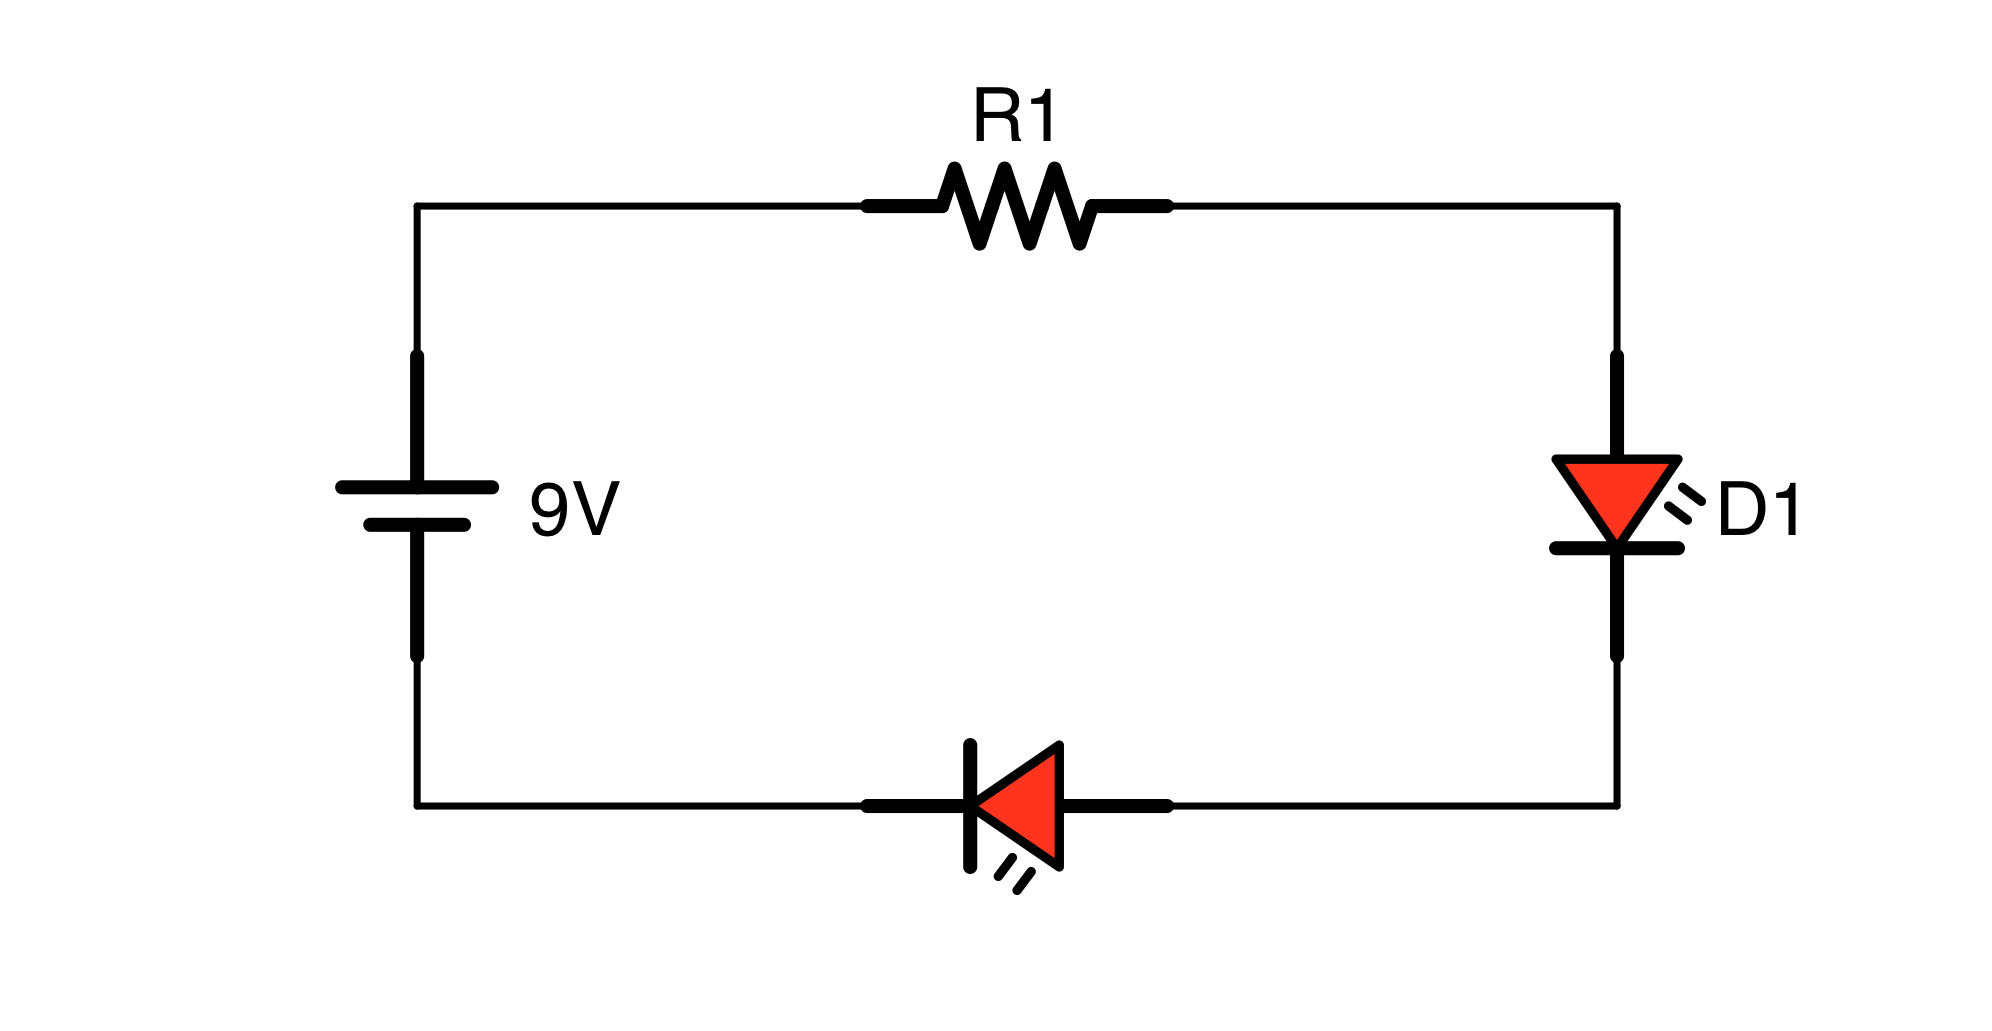
\includegraphics[width=\columnwidth]{SolutionTwoLED.png}
}
\end{enumerate}

